\documentclass{article}
\usepackage[margin=1.5cm]{geometry} % Change the margins
\usepackage[utf8]{inputenc} % - Defines what coding LaTeX uses. Use this one.
\usepackage[swedish]{babel}
\usepackage[T1]{fontenc}
\usepackage{graphicx} % - Package for including images in the document.
\usepackage{amsmath}
\usepackage{mathtools}
\usepackage{float}
\usepackage{caption} % Correct spacing for captions
\usepackage{siunitx} % Package for handling numbers (ex \num{1e6}), units (ex \SI{15,3}{Nm}) and intervals (ex\SIrange{10}{20}{\celcius}) correctly

\usepackage[style=numeric,backend=biber,sorting=none]{biblatex}
\DeclareLanguageMapping{english}{english-apa}
\addbibresource{references.bib}


\title{SysML 2.0 Viewer in a Browser}
\author{Oliver Högberg, \tt olihgb-7@student.ltu.se \\ 
Emma Carlsson, \tt emacar-8@student.ltu.se \\ 
Axel Kärnebro, \tt axekrn-7@student.ltu.se \\ 
Magnus Stenfelt, \tt magset-8@student.ltu.se \\
\\
\\
\\
\\
\\
\\
\\
\\
\\
\\

\includegraphics[width=0.3\textwidth]{ltu_swe.jpg}}
\date{December 2020}

\newpage

\begin{document}

\maketitle
\newpage
\tableofcontents
\newpage

\section{Introduction}

\subsection{Background}
When developing large systems it is very important to not lose understanding of the system, however it's also very hard to not lose it. This is why developers have used some kind of modelling languages throughout time. UML, Unified Modeling Language, is one such language and SysML, Systems Modeling Language, is an offshoot of UML and lets users practice Model-Based Systems Engineering(MBSE).  Modelling languages allows for creation of a graphical representation of the system, with varying levels of detail and complexity depending on what the project in question needs. It also allows developers to create and plan the entire system ahead of time, making it easier to avoid messy code and improves overall readability 
\\ \\
SysML v1 is a complete modelling language with very useful tools for creating and viewing system models. However there is a newer version of SysML in development, v2, which doesn't have any easy-to-use tools available for viewing system models. There are some tools, such as Eclipse Papyrus, but they are very complicated to install due to requiring many plugins and packages, and complicated to use making them unusable for less tech-literate users.
\\ \\
A proof of concept of an interactive SysML v2 viewer in a browser has been developed in a bachelor thesis here at LTU Jesper Nilsson in \cite{Jesper2020} proving that it is possible to render SysML diagrams in a browser. When another person took on the job \cite{Tommy2020} to build on the proof of concept as a summer job however, it was discovered that a proof of concept doesn't necessarily scale and their solution couldn't be pushed forward further. Additional work is required to restart the project from scratch to avoid these scalability issues. 
\\ \\
This is why this project was started, to find a way around the issues the prior experiments arrived at and to create a finished product, An interactive SysML v2 viewer in a browser.

\subsection{Problem description}
We have been tasked to create a web viewer for SysML v2. The viewer is meant to be for the system designer to use for a more clear and easy to understand description. There also has to be a tool to create the diagrams for SysML v2. After creating the SysML diagrams it is to be uploaded and shown in a clear and interactive manner. In the final product you are supposed to be able to click your way through on different parts to get to other diagrams giving the entire SysML more clarity. This is to be from a very high level overview and then ideally down to single components or parts of the entire system.
\\\\
The goal of this project is get an understanding of the SysML v2 language and in the end create an easy to understand tool for future SysML diagrams. We are also supposed to create this program in such a way that it can be built upon by another programmer in the case of us not succeeding. It also has to be able to be built upon due to SysML v2 not being finished and it still being updated. 
\\
In one sentence the project is to create a scalable SysML v2 web viewing tool that is easy to use and understand.

\subsection{Objectives}
The overall objective with this project is to create a tool which allows the user to get a clear understanding of a system. This tool should be able to give both an overview of the system and show the small details and how all the parts are connected. The system should be visualized using the SysML diagrams and written with the syntax of SysML v2 which is still in development. A very important part of this project is to make it open and scalable, our main goal is to lay the groundwork so that others can build upon and perfect it. 
\\\\
This shall be demonstrated at the end of the project by running an example project written in SysML v2 on our website which should be able to parse the code, display at least one diagram and be interactive in such a way that the user can navigate from one diagram view to another. This diagram should be either a block definition diagram, internal block diagram or a sequence diagram. 
\\\\
To reach this objective we need to make sure that we, as developers really understand what we are creating and that we have a sound and well thought through plan to avoid getting stuck. We also need to use the former attempts at this project to learn what worked and what to do differently in order to succeed.

\section{System design}

\begin{figure}[H]
    \begin{center}
        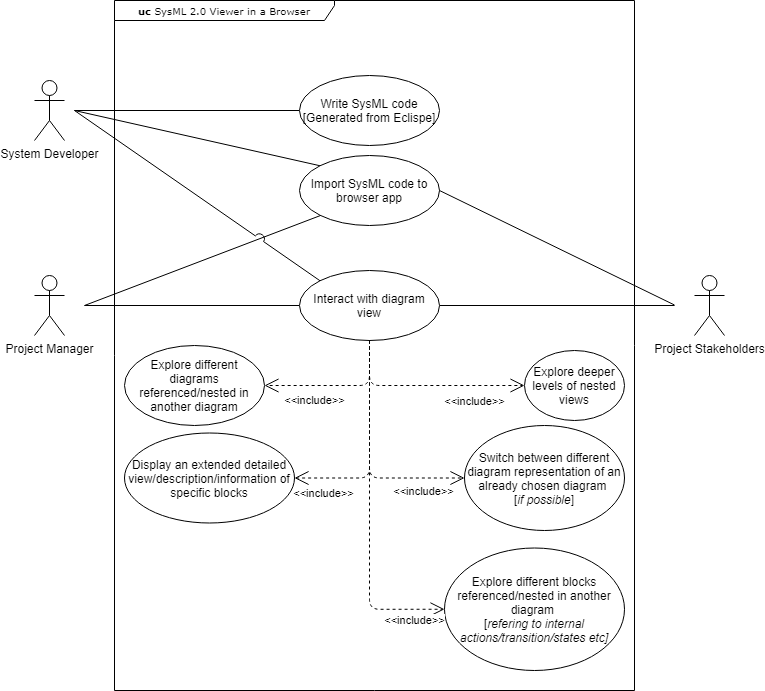
\includegraphics[width=0.7\textwidth]{Use-case_SysMLProject_first-draft.png}
        \caption{Use-case diagram describing some uses of the SysML interactions}
        \label{use-case}
    \end{center}
\end{figure}

The use-case diagram shown in figure \ref{use-case} describes the various uses of the solution for the primary actors: 
\begin{itemize}
  \item System Developer - The main function of this actor is as a developer and engineer of a particular system. 
  \item Project Manager - This actors main function is as the project lead of the particular system that is being developed. As a project manager this actor oversees the team of system developers and provides the communication channel with the project stakeholders.
  \item Project Stakeholders - This actors main function is that of an external (or in some cases internal) party which have interests of the particular system being developed. This actor can in a sense be seen as the customer of the particular system being developed.
\end{itemize}

\begin{figure}[H]
    \begin{center}
        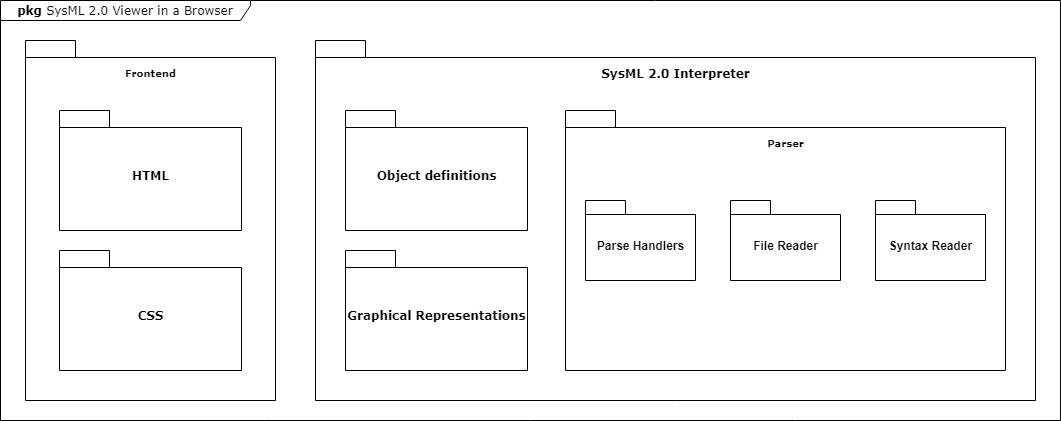
\includegraphics[width=1\textwidth]{Packages_SysML-Project_first-draft.png}
        \caption{Package diagram describing the basic structure of the implementation}
        \label{package}
    \end{center}
\end{figure}

The package diagram in figure \ref{package} shows the structure of our program. It consists of a frontend part and an interpreter. The frontend will be used to display a website using html and css presenting a graphical view of a system using SysML v2. 
\\\\
The interpreter consists of object definitions which handles the SysML v2 syntax that needs to be defined in order for the parser to translate the input correctly. The object definitions together with the parser is then used by the graphical representation to provide a graphical view of the parsed object definitions from the input. The parser in itself consists of the file reader, a syntax reader and the parse handlers. The parse handlers connects the parser with the object definitions so that a translation is possible while the file reader is responsible for actually reading the input and at last the syntax reader is responsible for interpreting what the file reader reads.


\printbibliography


\end{document}
